%% ---------------------------------------------------------------------------
%% Multimedia Systems (Springer) submission build.
%% Compile:  pdflatex main_sn ; bibtex main_sn ; pdflatex main_sn ; pdflatex main_sn
%% Bibliography style: sn-basic (Springer Basic, numbered) from paper/bst/
%% ---------------------------------------------------------------------------
\documentclass[pdflatex,sn-basic,Numbered]{sn-jnl}

\usepackage{graphicx}
\usepackage{booktabs}
\usepackage{amsmath,amssymb,amsfonts}
\usepackage{url}
%% Links stay clickable but are printed in black; sn-jnl defaults to blue.
\hypersetup{citecolor=black,linkcolor=black,urlcolor=black}
%% sn-jnl prints author e-mails with a hard-coded \textcolor{blue}; keep them black.
\makeatletter
\def\email#1{\global\advance\emailcnt by 1\relax
  \if@corauemail
    \g@addto@macro\corrauthemail{\setcounter{footnote}{0}\textcolor{black}{#1};\ }%
  \else
    \g@addto@macro\authemail{\setcounter{footnote}{0}\textcolor{black}{#1};\ }%
  \fi}
\makeatother

\renewcommand{\topfraction}{0.92}
\renewcommand{\bottomfraction}{0.92}
\renewcommand{\textfraction}{0.08}
\renewcommand{\floatpagefraction}{0.85}
\setcounter{topnumber}{3}
\setcounter{bottomnumber}{2}
\setcounter{totalnumber}{5}

\begin{document}

\title[Within-recording exposure in a slice-level reconstruction]{Within-recording exposure in a
slice-level reconstruction: an audit of a multi-library Chinese music information retrieval framework}

\author*[1]{\fnm{Yuan} \sur{Zhao}}\email{zhaoyuan@hist.edu.cn}
\author[2]{\fnm{Yingtao} \sur{Ji}}\email{jiyingtao@hist.edu.cn}
\author[2]{\fnm{Mengjie} \sur{Hu}}\email{hmj@hist.edu.cn}
\author[3]{\fnm{Songmei} \sur{Liu}}\email{liusongmei@xxgc.edu.cn}
\author[2]{\fnm{Chenyu} \sur{Yang}}\email{yangcy@hist.edu.cn}

\affil*[1]{\orgdiv{School of Foreign Languages}, \orgname{Henan Institute of Science and
Technology}, \orgaddress{\city{Xinxiang}, \postcode{453003}, \country{China}}}
\affil[2]{\orgdiv{School of Music and Dance}, \orgname{Henan Institute of Science and
Technology}, \orgaddress{\city{Xinxiang}, \postcode{453003}, \country{China}}}
\affil[3]{\orgdiv{School of Humanities and Law}, \orgname{Xinxiang Institute of Engineering},
\orgaddress{\city{Xinxiang}, \postcode{453003}, \country{China}}}

\abstract{\textbf{Purpose} Pre-computed spectrogram releases can obscure the unit of evaluation.
We audit the slice-level interpretation of CCMusic's stated split ratios, distinguishing our
reconstruction from the original authors' unavailable split files. \textbf{Methods}
Five mel-image libraries from the release, three of them among the six datasets the audited
article evaluates, contribute 110,415 slices from 7,827 recordings in 252 classes;
109,831 slices, 7,756 recordings and 234 classes meet our recording-level rules.
Three main arms compare clean training, equal-volume injection of held-out Q-pool slices, many
from recordings also represented in the test panel, and a random-slice reconstruction. An additional CTIS-only control injects non-test content.
We report paired recording-cluster bootstrap intervals conditional on the fixed split and trained
seeds, and supplementary class-stratified and joint seed--recording sensitivity analyses.
\textbf{Results} In CTIS, the A1--A0 pool-injection contrast changes macro-F1 by +2.02 points under AlexNet
(95\% CI +0.83 to +3.35) and +1.70 under Swin-T (+1.28 to +2.84).
Both intervals exclude zero; only the Swin-T interval lies wholly below the internally specified
three-point threshold. Recording-level estimates are +1.37 and +1.61 points; the exploratory
joint seed--recording interval for AlexNet includes zero. Against a matched control that injects the
same volume of non-test content, the contrast is +1.96 (+0.74 to +2.99) and +1.07 (+0.23 to
+1.96), so the difference between the two arms survives but is smaller than the A0 contrast.
Four additional libraries change by +8.4 to +28.7 points. Our reconstruction of the stated random
split changes CTIS by +1.21 (-0.02 to +2.44) and +1.75 (+1.18 to +2.70) points, and the self-test
score it would print is markedly higher than any sealed-panel arm; that score is illustrative and
is not the original benchmark score. Five of six near-single-slice control intervals include zero, with seed
signs that disagree and six contrasts reported without multiplicity correction; they check the
pipeline and do not establish equivalence. \textbf{Conclusion} Slice-level evaluation can reward within-recording
recognition. Our contrasts do not isolate pure memorisation from recording diversity.
Naming the split unit, reporting recording capacity and separating conditional inference from
training uncertainty makes benchmark scores more interpretable.}

\keywords{data leakage, benchmark audit, music information retrieval, reproducibility,
recording-level splits, mel spectrograms}

\maketitle

\section{Introduction}\label{sec:intro}

A benchmark number is only as informative as the split that produced it. When a dataset is
released as pre-computed spectrogram images, one image corresponds to a short window of one
recording, and a model trained on images from a recording has already seen the acoustics of
that recording: instrument timbre, room, performer, and microphone. A split over images can
therefore test within-recording recognition rather than generalisation to unseen recordings.
This is a case of non-independence between training and test, one category in the leakage
taxonomy of Kapoor and Narayanan~\cite{kapoor2023leakage}. The magnitude is an empirical
question; our paired audit measures it without changing the backbone.

Music information retrieval, or MIR, has dealt with this problem for a long time. Splitting by recording is
used in several audio benchmarks, for example urban sound, instrument and genre corpora, and the
split unit is usually stated explicitly; Salamon et al.~\cite{salamon2014urbansound} fixed a recording-level split for
UrbanSound8K in 2014, keeping slices of one recording within one fold so that evaluation is
recording-disjoint and comparable across papers. Yet datasets
that distribute features instead of audio make the split unit easy to lose, and multi-library
benchmarks, which pool heterogeneous sources under one evaluation protocol, make the loss hard
to notice: each library carries its own release format, its own file naming, and its own notion
of what one ``item'' is.

This paper audits one such framework. CCMusic \citep{zhou2025ccmusic} is a recent Chinese-music
resource whose associated article documents six datasets and evaluates all six under one
framework; the public release carries thirteen libraries under one publishing organisation, of
which those six are a subset. It distributes chroma, CQT and MEL features as pre-computed
images, and its evaluation framework states a split ratio for each collection --- 8:1:1 for
CTIS after 2-second segmentation, a recording-level 79:10:10 for Guzheng Tech99, 6:2:2 for
ErhuPT --- naming the split unit only in the recording-level case. We examine a
slice-level interpretation supported by the released format: MEL images are named by recording
and window index, and a naive 8:1:1 split over image filenames places windows of the same
recording on both sides. The released archives make this reconstruction possible, but do not
establish the split actually used by the original authors.

Our contribution is a measurement, not a discovery of a new phenomenon. The framework's own
documentation leaves three quantities unstated, and we estimate each of them. The first is the
size of the A1$-$A0 contrast under equal-volume replacement with matched training-pool
recording counts, while acknowledging that A1 introduces additional pool recordings. The second is whether a recording-level split is feasible for these libraries at their
stated class counts, given that splitting by recording consumes recordings that would otherwise
train the model. The third is whether the pipeline yields small contrasts in near-single-slice controls,
where homologous exposure is absent or very limited by construction.

To answer them we rebuilt the five libraries that release MEL slices --- 110{,}415 released
images from 7{,}827 recordings across 252 classes, of which 109{,}831 images from 7{,}756
recordings across 234 classes survive a minimum-recording rule --- under a recording-level
three-way split, and trained two standard backbones, AlexNet and Swin-T, under three main arms.
A CTIS-only fourth arm, C1, was added to check equal-volume non-test injection. The control arm, A0, samples a fixed number of
slices per class from the training recordings and never touches a test recording. The exposure
arm, A1, injects the entire held-out Q pool by equal replacement. Many pool slices come from
recordings also represented in the test set, but not all do; realised overlap is reported in
Supplementary Material S1. The number of training slices is held fixed and the
number of training recordings drawn from the training pool is matched. A1 differs from A0 in
whose content reaches training and in the additional pool recordings, whose counts are reported
per class; the contrast is therefore consistent with an advantage associated with
within-recording exposure, but it does not isolate one. A2 provides an illustrative self-test
score under our reconstruction of a slice-level split over the pooled corpus; it is neither a
reproduction of the original authors' unknown split files nor the original benchmark score.

Three results organise the paper. Conditional on the fixed split and the trained seeds, the
exposure arm gains $+2.02$ points of macro-F1 in the primary library, with a 95\% CI of $+0.83$ to $+3.35$, and $+1.70$ under
Swin-T with CI $+1.28$ to $+2.84$. Both intervals exclude zero. The Swin-T interval
lies wholly below our three-point smallest effect of interest;
the AlexNet interval includes three points, so that magnitude is not excluded. A CTIS-only
control arm that supplies the same volume of training slices from non-test content, C1, moves
the point estimate by $+0.05$ and $+0.62$ points only; measured against C1, the exposure arm
still gains $+1.96$ points $[+0.74,+2.99]$ under AlexNet and $+1.07$ $[+0.23,+1.96]$ under
Swin-T, so the difference is smaller than the A0 contrast, though its paired interval excludes zero under
the fixed split and the trained seeds. In four other libraries
the same manipulation moves macro-F1 by $+8.4$ to $+28.7$ points. In the three negative-control
libraries --- near-single-slice collections --- five of six contrasts include zero. The sixth,
chest falsetto under Swin-T, is $-2.53$ $[-5.00,-0.21]$; its three seed-specific deltas are
$+5.57$, $-2.62$ and $-10.54$ points, so the sign is not stable across seeds. With six
contrasts and no correction for multiplicity, these controls check the pipeline, not the
mechanism in isolation, and they do not establish equivalence.

We are careful about what these numbers license. They do not show that CCMusic is
irreproducible, nor that its authors made an error that invalidates published results: the
audited article is a database paper, and its evaluation framework is one section of it. They do
show a small positive equal-replacement contrast in CTIS and larger contrasts in four additional
libraries, conditional on our fixed reconstruction and training recipe. They also give the
arithmetic needed to judge whether a recording-disjoint split is feasible at the stated
per-class requirements, rather than treating feature images as independent examples.

The remainder of the paper is organised as follows. Section~\ref{sec:related} positions the
audit against leakage taxonomy, audio-dataset practice, and dataset audits in adjacent fields.
Section~\ref{sec:framework} states what the audited framework says and what its released files
imply. Section~\ref{sec:materials} describes the five libraries, the manifest, and the
capacity calculation. Section~\ref{sec:protocol} defines the arms, the sealing protocol, and
the statistical plan. Section~\ref{sec:results} reports the main effect, the random-split arm,
the negative controls, and a cross-instrument experiment on one library.
Section~\ref{sec:discussion} discusses what the size of the effect depends on and what a
reporting standard should require. Section~\ref{sec:conclusion} concludes.

\section{Related work}\label{sec:related}

\subsection{Leakage as a reproducible failure mode}

Kapoor and Narayanan~\cite{kapoor2023leakage} catalogue leakage across machine-learning-based science and give it
a working taxonomy: leakage occurs when information that would not be available at prediction
time enters training, and it is dangerous precisely because the result looks better rather than
worse. One of their categories, ``non-independence between train and test'', covers our case
directly: two rows derived from the same underlying unit are not independent, and a random
split over rows therefore delivers an optimistic estimate of generalisation. The same
diagnosis has been made in recommendation \citep{ji2023leakage}, where offline evaluation
routinely mixes user interactions across the split, and in translational
EEG \citep{brookshire2024eeg}, where segments of one recording are treated as separate samples. The phenomenon also has a data-mining formulation: leakage arises when a feature is generated
after the target and therefore carries information about it \citep{kaufman2012}. Our case is a
different mechanism with the same consequence. The window is not generated after the label; it
comes from the same recording, so a training row and a test row can be two views of one
performance and are not independent draws.

The methodological implication is that the unit of splitting must be named and, when the release
format makes rows rather than units look atomic, verified against the files. A benchmark that
releases feature images falls into exactly this trap, and the trap is silent: the pipeline runs
without error, the score looks plausible, and only the split unit distinguishes an optimistic
number from a transferable one.

\subsection{Splitting practice in audio}

Recording-level separation is an established practice in audio evaluation. Slice- or chunk-level
partitioning can expose a model to siblings of test examples, making within-recording recognition
possible rather than ensuring transfer to new recordings. Salamon et al.~\cite{salamon2014urbansound}
formalised this for urban sound, fixing ten folds at the recording level so that folds are
comparable across papers. Corpora that share the practice differ in what they document as the
splitting unit rather than in a single convention: FMA fixes an 8:1:1 partition at the recording
level \citep{defferrard2016}, whereas tagging and transfer studies built on curated track-level
collections report track identifiers instead \citep{choi2017,lee2017,won2020}, and shared
evaluation campaigns have made cross-paper comparison routine \citep{downie2010mirex}; CCMusic
extends this landscape to a multi-library Chinese-music resource \citep{zhou2025ccmusic}.
GiantMIDI-Piano is instead a large classical-piano MIDI resource \citep{kong2022giantmidi}.
Environmental-sound datasets and augmentation studies provide useful evaluation recipes
\citep{piczak2015,salamon2017augment}; we do not take them as evidence that augmentation
quantitatively removes, or fails to remove, leakage. The
difficulty is sharpest for collections distributed as pre-computed features: the audio may or may
not accompany the images, the file names encode windows, and new users inherit whatever split the
release implies.

\subsection{Released representations and what they cost}

Release formats changed as audio models grew. Large annotated corpora of audio events and music \citep{gemmeke2017audioset,engel2017} made it attractive to publish embeddings or spectrograms instead of waveforms \citep{hershey2017cnn,kong2020panns}, and self-supervised audio models now ship representations that downstream users fine-tune rather than retrain \citep{elizalde2024clap,li2023}. Each of these releases moves the split decision upstream: whoever pre-computes the features also decides what an item is, and a downstream user who sees one image per row has no reason to suspect that rows are windows.

\subsection{Dataset audits}

Auditing a published dataset is an established genre. Sturm~\cite{sturm2012gtzan} showed that a
widely used genre benchmark contains mislabels and duplicates that change conclusions drawn
from it. Our audit differs in object: we do not question the content of the labels or the
duplication structure of the corpus, but the protocol that maps that corpus onto train and test.
Audits of this kind have a second, sharper form: a system can be shown not to listen at all, in which case the benchmark measures the shortcut rather than the task \citep{sturm2014horse}. Re-measuring a leaderboard number under a different protocol and finding that it moves is likewise an established result \citep{recht2019}, and dataset documentation now asks authors to state the split unit rather than leave it to the reader \citep{gebru2018}. That distinction matters for how the result should be read --- a labelling defect is a property
of the data, whereas a split-unit defect is a property of the evaluation recipe and can be
repaired without re-collecting audio, provided recording identifiers are recoverable and
each class retains enough independent recordings, the condition our capacity calculation checks.

\subsection{What is new here}

To our knowledge, score inflation under slice-level splitting and the feasibility of a
recording-level split have not been jointly quantified on a multi-library Chinese MIR benchmark.
Our three main arms control training volume while varying content origin; the CTIS-only C1
control probes non-test replacement. These controls narrow the interpretation, but do not fully
separate content identity from recording diversity.

\section{The audited framework and what its split implies}\label{sec:framework}

\subsection{The release}

CCMusic \citep{zhou2025ccmusic} is a Chinese-music resource whose associated article documents
six datasets, from instrumental technique corpora to popular-song excerpts, and evaluates all six
through one framework. The release we audited is larger than the article: it comprises thirteen
library directories published under the same ModelScope organisation, of which the six datasets
described in the article are a subset. Each library ships chroma, CQT and MEL features computed
from the audio, stored as one image per short-time window; the article notes that the MEL
spectrogram is provided alongside the audio for visualisation. The evaluation framework pools
datasets that share a task and trains a common classifier per task. We checked the version of
record in TISMIR 8(1), pp. 22--38 (2025), against the arXiv release and against the archives we
downloaded on 2 November 2026. On printed p. 26 the article states, for CTIS, that the dataset
was randomly split into training, validation and testing sets at a ratio of 8:1:1 after
2-second segmentation, at 43{,}054 clips, without naming the split unit; p. 28 gives a
recording-level 79:10:10 split for Guzheng Tech99, p. 29 a 6:2:2 ratio for ErhuPT without naming
the unit, and the remaining collections are given only an 8:1:1 ratio. No recording-group
constraint is attached to the stated evaluation protocol. This supports auditing the slice-level
interpretation where the statement names no unit, but does not recover the original authors'
actual split files.

Two properties of the release shape the audit. First, the feature images are the unit of
analysis: for the MEL family, each image is a 496$\times$369 JPEG whose file name encodes the
recording identifier and the window index. What ships beside the images also differs in what can be checked: all five libraries release
source audio, but only in CTIS do the audio file names map unambiguously onto the evaluation
recording identifiers, so the five libraries in Table~\ref{tab:panels} are not equally checkable
against the audio. Second, the
same recording contributes many images --- between 8.7 and 48.9 per recording across the five
libraries we use, as Table~\ref{tab:panels} lists --- so the number of images per recording is large
enough for a slice-level split to place many siblings of every test recording in training.

\subsection{The split statement}

The framework states that each dataset is ``randomly split \ldots at a ratio of 8:1:1''. The
statement does not name the unit of splitting, and the released files support a slice-level
reading: a split over image files. We verified that the article states no grouping constraint
in the stated evaluation description --- by recording, song, performer or album. Under the slice-level reading almost every test slice has siblings in training. If the
80/10/10 split is drawn independently per slice, then conditional on one slice of a recording
sitting in the sealed panel, the probability that at least one of its remaining $K-1$ slices
lands in training is $1-0.2^{K-1}$, since each sibling avoids the 80\% training share with
probability 0.2. It is 0.99999744 at $K=9$ and exceeds 0.999999999 at $K=14$ and $K=21$.
This is an independent-allocation calculation, not an exact formula for a fixed-size,
without-replacement partition. The
unconditional probability that a recording of $K$ slices contributes at least one training slice
is $1-0.2^{K}$. Figure~\ref{fig:units} contrasts the two units on one recording in its top two rows, and then
shows how the pool moves between panels in its bottom two rows.

\begin{figure}[!t]
\centering
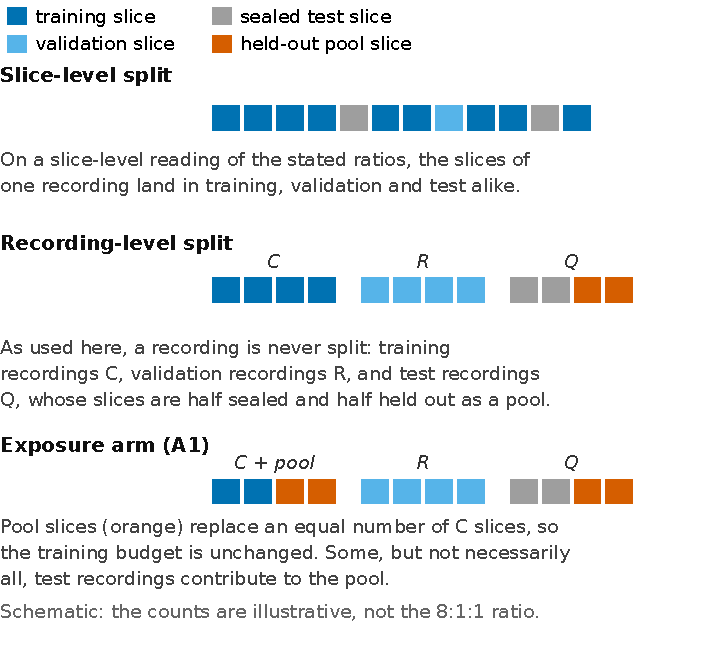
\includegraphics[width=\linewidth]{../figures/fig1_split_units.pdf}
\caption{Split units and the exposure intervention (schematic, not an exact 8:1:1 allocation).
Top: a slice-level partition can place siblings in training, validation and test. Middle: the
recording-disjoint allocation assigns training recordings to C, validation recordings to R,
and test recordings to Q; Q is then divided into sealed $Q_{\mathrm{test}}$ and
held-out $Q_{\mathrm{pool}}$ slices. Bottom: A1 replaces C slices with
$Q_{\mathrm{pool}}$, while $Q_{\mathrm{test}}$ remains sealed.}
\label{fig:units}
\end{figure}

We treat this as a specification question rather than an accusation. A database paper can leave an evaluation detail underspecified without establishing that its
implemented split was defective. We therefore distinguish the stated recipe, our slice-level
reconstruction, and the unavailable original split files. What the audit adds is the size of the gap between the protocol as stated and the protocol a
reader would need to interpret the number as generalisation to unseen music. The exposure
distribution, the capacity calculation and the four-arm contrast support that gap jointly; A2
contributes only a slice-level approximation.

\subsection{Terms}

We use \emph{recording} for the unit that a split should respect, meaning one performance or one
file in the source collection, \emph{slice} for one released feature image, $\bar K$ for the mean
number of slices per recording in a library, and \emph{homologous content} for the slices of a
recording whose other slices are in the test set. The implemented Q pool can also contain
recordings without test slices because grouped allocations need not put every recording on both
sides; A1 injects the full pool, not solely the homologous subset. A recording-level split is one in which all
slices of a recording fall on the same side of the partition.

\section{Materials}\label{sec:materials}

\subsection{Five libraries with released MEL slices}

We use the five collections for which the MEL family is released with per-class labels and more
than one slice per recording: CTIS for Chinese instrument recognition, music genre for
popular-song excerpts, pianos for eight piano brands, CNPM for Chinese pentatonic-mode classification, and
bel canto for bel-canto and folk singing. Three of the five --- CTIS, CNPM and bel canto --- are
among the six datasets evaluated in the audited article; \emph{music genre} and \emph{pianos}
belong to the same published collection of libraries but are not covered by it, so contrasts in
those two libraries audit the same kind of split under a framework that does not report on them.
Together they release 110{,}415 slices from 7{,}827 recordings in
252 source classes; folding the duplicate takes described below leaves 7{,}825 canonical
recordings, which is the footing of the library inventory in the supplement. Of these,
109{,}831 slices from 7{,}756 recordings in 234 classes survive the
minimum-recording rule and placeholder removal described in
Section~\ref{sec:capacity}, listed in Table~\ref{tab:panels}; the remainder is excluded under
these study-specific rules. In CTIS the rule leaves 42{,}509 of the 43{,}054 released slices in
201 classes, and four of those slices repeat a content hash already claimed by the sealed panel,
because the same take is released under two technique names; those four are dropped when the
partitions are built, so the four partitions carry 42{,}505. The four candidate near-single-slice collections are not part of the main sample; three are used
as controls and the fourth is excluded for lack of a usable class layer, as described
in Section~\ref{sec:protocol}.

\begin{table}[t]
\centering
\caption{The five audited libraries after manifest construction and recording-level splitting,
i.e.\ the sample every reported number is computed on. Classes are the source classes that
survive the minimum-recording rule; $\bar K$ is the mean number of slices per recording;
$Q_{\text{test}}$ is the sealed panel; $\alpha$ is the realised exposure ratio
$Q^{\text{pool}}_c/m_c$, summarised by its median over classes (not the pooled ratio).
Counts are those of the frozen partition files, so a take released twice under two technique
names is counted once.}
\label{tab:panels}
\footnotesize
\setlength{\tabcolsep}{3.4pt}
\begin{tabular}{lrrrrrrr}
\toprule
Library & Classes & Recordings & Slices & $\bar K$ & $Q_{\text{test}}$ sl. & $Q_{\text{test}}$ rec. & $\alpha$ \\
\midrule
CTIS            & 201 & 4{,}887 & 42{,}505 &  8.70 & 4{,}605 & 963 & 0.160 \\
music genre   &  16 & 1{,}713 & 36{,}375 & 21.23 & 3{,}648 & 337 & 0.166 \\
pianos          &   8 &   668 & 18{,}352 & 27.47 & 1{,}884 & 135 & 0.170 \\
CNPM            &   5 &   286 &  2{,}713 &  9.49 &   271 &  54 & 0.161 \\
bel canto     &   4 &   202 &  9{,}886 & 48.94 &   979 &  40 & 0.161 \\
\midrule
Total           & 234 & 7{,}756 & 109{,}831 & 14.16 & 11{,}387 & 1{,}529 & --- \\
\bottomrule
\end{tabular}
\end{table}

\subsection{Recording identity}

Every slice is mapped to a \texttt{recording\_uid} by a rule specific to the library, derived
from the release format: CTIS by the
per-class file stem, prefixed by the class code when a stem repeats across classes;
music genre by the pair of track index and duration that the file name encodes; pianos by brand,
recording number and duration; CNPM by joining the file name to the dataset's own
\texttt{label.csv}; and bel canto by class and recording number. The identity field parsed for
all 110{,}415 slices; the separate instrument-name field parses
for 99.49\% of CTIS slices, and the 14 unparsed stems are reported in the manifest summary.
We obtained the audio archives of CTIS, CNPM and pianos. Audio-level verification of these
identities was possible only for CTIS, the one library whose audio file names map unambiguously
onto its evaluation recordings; in CNPM and pianos the audio file names carry no reliable link
to the evaluation recording identifiers, so their identities rest on the file-name rule alone.
Bel canto and music genre also release audio, which we did not obtain. A correct parse is in any case not the same as a correct identity: the rule can
reproduce a plausible recording identifier without proving that the released images and the
released audio belong together.

Two checks protect the mapping. First, the mapping between a CTIS recording and the numbering of
its slices is a global counter over classes, not a per-class index; using the per-class index
mis-assigns 218 of 219 classes, and the manifest builder recomputes the global counter before
joining. Second, a SHA-1 sweep over all 4{,}956 CTIS files, 13.3 GB, found two identical pairs --- one take
released under two technique names, and one take with a duplicate-download suffix ---
which we fold to a single canonical identifier carrying one label, so that no canonical
recording appears in two classes and none can sit on two sides of a split by accident. At the slice level CTIS holds 77 groups of identical images,
covering 175 slices. In every one of them the same window appears under more than one recording
name: in 51 groups those names resolve to one recording's audio after the SHA-1 folding above, and
in 26 they resolve to two or more distinct recordings, so the group key rather than the recording
name is what keeps the copies on one side. Separately, in music genre one group of identical
images spans three classes. Within the sealed panel and the exposure arms, every such group is
forced to a single side.

\subsection{Capacity for a recording-level split}\label{sec:capacity}

Capacity planning targets $q_c=\min\{\max(5,\mathrm{round}(0.2n_c)),n_c-1\}$
recordings and $m_c^{\text{plan}}=0.60S_c$ slices. The implemented split also reserves R:
it starts from $\max(1,\mathrm{round}(0.15n_c))$ validation recordings, selected to
approximate $0.15S_c$ slices while retaining the training budget. It starts Q from
$\min\{\max(5,\mathrm{round}(0.2n_c)),n_c-2\}$ recordings, reduces Q when necessary to
leave C non-empty and large enough, and flags these relaxations per class.
The planning half-pool approximation is $\sum_{i\in Q}\lfloor k_i/2\rfloor$;
it is not the exact implemented allocation. Within each selected Q recording, adjacent slice
pairs are joined, and groups sharing an image content hash within the same class are joined
further. Every group is keyed by the smallest content-derived identifier among its members --- a
string formed from the first twelve hexadecimal digits of the slice's SHA-1 --- so the key
depends on image content only, never on time, class or label. Groups are sorted by that key and
assigned alternately to sealed test and injection pool, with singleton groups forced to the test
side and any further copy of an already assigned hash following it. This is neither a contiguous
time half nor independent random assignment; group ordering and duplicate constraints determine
realised pool size.
The realised
exposure ratio $\alpha_c = Q^{\text{pool}}_c/m_c$ is largely determined by design:
a 20\% recording test share, approximately half of its slices in the pool, and a
$0.60S_c$ training budget give $\alpha\approx0.2\times0.5/0.6=0.167$.
Rounding, class support, slice multiplicity and duplicate constraints cause deviations; its median lies between 0.160 and 0.170 in every library, and its per-library span
is 0.000--0.250 for CTIS, 0.162--0.168 for music genre, 0.161--0.173 for pianos, 0.154--0.175
for CNPM and 0.158--0.170 for bel canto. Earlier 50\% and 30\% replacement targets are
capacity questions, distinct from realised exposure. A planning calculation using the upper
95th-percentile pool over repeated draws gives 24 and 54 feasible classes among 219 source
CTIS classes; restricted to the 201 analysed classes these counts are 10 and 38.
These upper-capacity counts do not mean that the frozen split realises such exposures.
CNPM selects 57 recordings for Q, but only 54 contribute sealed test slices: the other three
have all their selected groups allocated to the pool. Table~\ref{tab:panels} counts
recordings actually represented in the test panel.

Two consequences shape the design. First, equal replacement, not addition: injecting
$Q^{\text{pool}}_c$ slices while keeping $m_c$ fixed removes exactly as many C slices as it adds,
so the arms differ in composition and not in size. Second, the training-recording count must be
matched on the C side: A0 and A1 draw their training recordings from C, and matching the total
training-recording count across arms is impossible once A1 must also include pool recordings, so
we match the C-side count exactly and report the A1 total, C side plus pool, per class. Where
the C side cannot supply the planned budget the realised $m_c$ is capped at what C holds, and
where a class cannot yield the planned $q_c$ the pool is trimmed; both events are flagged per
class in the released feasibility table, so a reader can see exactly where the arithmetic binds.

We required at least five recordings per class as a study-specific eligibility rule; this is not a
mathematical minimum for every possible recording-level split. Applying that rule to CTIS reduces 219 source
classes to 206. Five further classes (D0051, D0058, D0060, D0061 and D0062) each contain
one placeholder recording whose identifier includes a Chinese ``no audio'' marker; removing it reduces
five recordings to four in each class, giving 201 classes and 4{,}887 recordings. The placeholder
slices in D0060--D0062 share a byte-identical set of 21 images; D0051 and D0058 have 27 and 26
placeholder images, respectively. Supplementary Material S1 lists the class-level exclusions. The other four libraries keep
all their classes; two of them lose one recording each, because duplicate removal took every
slice of that recording, leaving CNPM with 286 of 287 and bel canto with 202 of 203, while
pianos and music genre lose nothing. We report both counts wherever the source documents state 219, so that the
difference between the released class count and the auditable one is visible rather than
implicit.

\subsection{Feature cache}

All five libraries release MEL images at 496$\times$369. We resize to 224$\times$224 with
bilinear interpolation and store the result as a \texttt{uint8} memmap in manifest order: the
109{,}831 audited images plus the excluded classes come to 15.48 GiB for the five libraries, and
the 5{,}432 negative-control images add 0.76 GiB. Aspect ratio is deliberately not preserved: the source
images share one size here, but across the full release the aspect ratios span two orders of
magnitude, and padding to a common shape would turn padding fraction into a library-level
covariate. A random sample of 200 images per library was re-decoded and compared with the cache
byte for byte: the maximum absolute difference is zero for all eight libraries.

\section{Protocol}\label{sec:protocol}

\subsection{Three main arms and a CTIS-only injection control}

A0 and A1 use the same per-class slice budget and are evaluated on the same sealed panel.
A2 approximates that budget through its random partition; C1 is an additional CTIS-only control,
not a fourth arm run across all five libraries.

\begin{description}
\item[A0, control.] For each class, sample a realised budget $m_c$ close to the planned
$0.60\,S_c$ slices from $r_c^{C}$ distinct recordings in C, the training partition, which contains no slice of a test recording. Nothing the model sees
shares a recording with anything it is scored on.

\item[A1, homologous exposure.] Same $m_c$ and same C-side recording count, but the entire
$Q^{\text{pool}}_c$ is injected and an equal number of C slices is removed. Much of this pool
shares recording identifiers with the sealed panel, but some pool recordings contribute no test
slices. Realised overlap is given in Supplementary Material S1; $\alpha_c$ is the full injected
pool fraction, not the fraction restricted to recordings represented in the test panel. In one
class, the suona technique cell C0296, four candidate pool slices repeat content that already sits
in the sealed panel and are removed by the duplicate-content rule before injection, so A1 trains
on four fewer slices than A0 and C1 (25{,}498 against 25{,}502) and the per-class budgets are equal
everywhere else.

\item[A2, slice-level reconstruction.] Draw the slice-level 80/10/10 partition of C $\cup$
$Q^{\text{pool}}$, i.e.\ a slice-level interpretation of the audited protocol, including same-recording
mixing. Training uses 80\% of that union; because the union is about $0.75\,S_c$, A2 trains on about
60\% of the original corpus. That shortfall is the price of matching the budget: the realised
training count lands within one percent of $m_c$ in every library, as Table~\ref{tab:a2} shows. A2 also
reports a self-test score on its own 10\% held-out share, which is an illustrative self-test score
under our reconstruction of a slice-level split over the pooled corpus; it is neither a
reproduction of the original authors' split nor the original benchmark score.
\item[C1, non-test injection (CTIS only).] Starting from A0, remove 4{,}177 slices and
replace them classwise with 1{,}665 slices from unused C content and 2{,}512 from R, all from
non-test recordings. Injection is disjoint from A0 samples, test samples, test recording IDs
and test content hashes. Realised counts equal A0 classwise, so the two arms
differ only in which slices are trained on; the total is 25{,}502, four more than A1's
25{,}498.
C1 uses seeds 0--2 and the same final-epoch recipe. Because it consumes R content, its
validation scores cannot be interpreted; it performs no validation-based selection.
This exploratory addition holds volume approximately fixed but not recording diversity.
\end{description}

A0 and A1 hold the number of training slices and the C-side recording count fixed, so a
difference between them cannot be attributed to more data or to more recording diversity within
C. What differs is whose content the model sees. A2 varies both mechanisms at once and therefore
serves as a plausibility check rather than as a third estimate of the same quantity.

\subsection{What the contrast estimates}\label{sec:estimand}

We state the estimand explicitly, because the arms differ in more than one respect.
The treatment condition replaces $|Q^{\text{pool}}_c|$ of the $m_c$ C slices with the whole
$Q^{\text{pool}}_c$ of the same class, keeping the budget at $m_c$; the control condition draws
$m_c$ slices from C.
Fixed across the two arms are the per-class slice count, the per-class count of C-side training
recordings, the epoch count and the resulting optimiser steps, as reported in Supplementary Material~S1, the sealed evaluation panel, the three training seeds and
the per-class label set. What the treatment changes is the number of pool recordings that reach
training, the identity of the content they carry, and the within-class diversity those recordings
add: on CTIS, 578 of 963 test recordings are represented in A1 training and none in A0.
We therefore call $A1-A0$ the \emph{pool-injection contrast} $\Delta_{\text{pool}}$ and read it as
the score change associated with injecting the held-out pool under an otherwise fixed budget.
It is not the effect of moving from a recording-level to a slice-level partition, because that
move also repartitions the pool; A2 is the arm that approximates such a move.
Table~\ref{tab:arms} summarises what each arm trains on.

\begin{table}[t]
\centering\footnotesize\setlength{\tabcolsep}{4pt}
\caption{What each arm trains on in the primary library (CTIS, 201 classes, 963 test
recordings). Recordings are distinct canonical identifiers contributing at least one training
slice. The per-class budget $m_c$ is identical in A0 and C1; A1 is four slices short in class C0296.}
\label{tab:arms}
\begin{tabular}{@{}llrrll@{}}\toprule
Arm & Training content & Slices & Recordings & Budget & Test-recording relation\\\midrule
A0 & C only & 25{,}502 & 3{,}017 & $m_c$ & disjoint, 0/963\\
A1 & C + all $Q^{\text{pool}}$, equal budget & 25{,}498 & 3{,}770 & $m_c$ & 578/963 shared\\
A2 & 80\% of $C\cup Q^{\text{pool}}$, slice level & 25{,}263 & 3{,}679 & $\approx m_c$ & same-recording mixing\\
C1 & C remainder + part of R & 25{,}502 & 3{,}684 & $m_c$ & non-test R, 0/963\\\bottomrule
\end{tabular}\end{table}

\subsection{Training and sealing}

The recipe is frozen: 224$\times$224 input, ImageNet initialisation, ten epochs, AdamW with
learning rate $3\times10^{-4}$ and weight decay 0.05, cosine schedule with one warm-up epoch,
label smoothing 0.1, batch size 64, and two backbones --- AlexNet \citep{alexnet2012} and
Swin-T \citep{swin2021} --- under three seeds.
No data augmentation is applied: the recipe specifies none, and time-axis flips are not
meaningful for spectrograms. The number of epochs is fixed at ten and the final-epoch weights are
the ones evaluated: no checkpoint, epoch or seed is chosen on any panel, so the reported scores
carry no selection step, and the validation partition is monitored and reported but never used to
pick a model.

The sealed panel is evaluated once per run, after training, and never during it. Per-seed
predictions are written to a staging directory and moved into a sealed directory only when all
seeds of a library--arm--backbone group have completed; the sealed record contains the
group's seed spread. This local record is not an independent timestamp and does not by itself
prove when analytical choices were made. No model, epoch or seed selection is performed; R contains no test
recording and is used for monitoring only, except that C1 consumes part of R as described above. This is what makes the reported differences interpretable: a
pipeline that peeked at the sealed panel to choose a checkpoint would produce a number that no
longer measures transfer.

\subsection{Metrics}

The primary metric is macro-F1 on the sealed panel. We compute it at two levels. At the slice
level, each slice is one prediction. At the recording level, the predicted probabilities of all
slices of a recording are averaged and the recording receives one label, which gives every
recording the same weight within a library and keeps a library with $\bar K = 48$ from dominating
one with $\bar K = 8.7$ through sheer slice count. Both levels are reported side by side; the
primary contrast is at the slice level, as specified in the internal analysis plan, and the recording level
serves as a robustness check, with any disagreement between the two flagged in the text. Macro-averaging is a reasonable summary when class support is uneven; we take the
motivating argument from the literature on precision--recall summaries under imbalance \citep{saito2015pr}, though that argument concerns two-class problems and we do not treat it as a general justification. Macro-F1 averages only over classes with non-zero support or
predictions in the evaluation panel. In the reported intervals the class set is recomputed within
each resampling replicate: a class that is absent from a replicate is dropped from that
replicate's mean rather than scored as zero. Supplementary Material S1 reports the variant in
which the class set is fixed once at the panel level and absent classes score zero; the point
estimates are identical and the intervals differ by less than half a point.

\subsection{Statistics}

Differences are paired at the slice level: for a given library and backbone, all arms are
scored on the same slices, which we verify by comparing the label and recording arrays of the
sealed records element by element. Intervals come from 2{,}000 bootstrap resamples of test
\emph{recordings}, with whole recordings resampled and the same resampling indices applied to
every arm and backbone. These intervals describe test-recording resampling uncertainty
conditional on the realised split and the three trained seeds; they do not include uncertainty
from new training seeds or a new train/test split. Concretely, let $f_{s,a,b}$ be the macro-F1 of seed $s$, arm $a$ and
backbone $b$ on the sealed panel. A reported arm score is the mean over seeds,
$\bar f_{a,b} = \frac{1}{3}\sum_s f_{s,a,b}$, and a reported effect is
$\hat\Delta_b = \frac{1}{3}\sum_s (f_{s,A1,b} - f_{s,A0,b})$, so the printed arm columns,
rounded to four decimals, need not subtract to the printed effect. Within each bootstrap
replicate the per-seed paired difference is recomputed from the stored per-slice predictions and
the replicate value is the mean over seeds; the interval is the 2.5--97.5 percentile range and
the tail proportion is a two-sided smaller-tail resampling measure obtained by inverting the
percentile interval, not from a null distribution. The original script clipped
zero-tail estimates to $1/B$; the reported analysis uses the add-one convention
$2(k+1)/(B+1)$ for the smaller-tail count $k$, capped at one, with $B=2{,}000$.
Its minimum raw value is $2/2{,}001$, not evidence of an exact tail probability. Because the class set is fixed by each dataset rather than sampled from a population of classes, these intervals describe resampling uncertainty over test recordings within the realised split and do not extend to unseen classes or to other libraries.
Seed dispersion is reported as the range over
seeds and is not tested: three seeds are too few to estimate between-seed variance reliably,
so the primary intervals treat them as fixed and seed dispersion is descriptive. A supplementary
class-stratified recording bootstrap and joint seed--recording bootstrap assess sensitivity;
resampling three seeds does not replace additional training or split realisations.

The internal plan designates a primary family of two tests: CTIS under AlexNet and CTIS under Swin-T, both for
A1$-$A0. There is no independent public timestamp verifying when the plan was fixed. We correct within that family by Holm's method at $\alpha = 0.05$. The smallest effect
of interest, or SESOI, is the three-point macro-F1 threshold recorded in the internal plan.
It is a study-specific practical decision threshold, not a significance cutoff and not an
externally validated minimum useful gain. Precision does not justify practical importance.
The other four libraries are additional, non-confirmatory applications of the same operation,
not replications of an identical task. No public preregistration was made; Supplementary
Material S1 distinguishes the internal plan, execution changes and post hoc analyses.

\subsection{Negative controls}

If the mechanism is homologous content, libraries whose recordings contribute one slice have
nothing to inject: $Q^{\text{pool}}_c = \sum_i \lfloor k_i/2 \rfloor = 0$ in every class, so the
exposure arm coincides with the control and A1$-$A0 is not identifiable. The only arm that can
then differ is A2, which also changes the random partition; we therefore report A0 and A2 with three
seeds on three collections --- chest\_falsetto with 1{,}280 recordings of one slice each,
erhu\_playing\_tech with 1{,}253, and GZ\_IsoTech with 2{,}824 recordings, 2{,}899 slices and 46 recordings
with two to four segments --- and read the contrasts as a pipeline sanity check rather than a test of the main intervention.
The expansion from the initial single-seed controls to three seeds is exploratory and is
listed in Supplementary Material S1.

Guzheng\_Tech99 is excluded from the control runs: every recording contributes one slice, and
the release carries per-note technique annotations whose per-recording dominant label is the same
technique \emph{boxian} in all 99 recordings, so no recording-level class layer exists. GZ\_IsoTech
is kept, and its exposure is not exactly zero: 46 multi-segment recordings put nine slices into
the pool under one random draw, an exposure of 0.005, against an expectation of 0.0065 under 400 draws with a 95th
percentile 0.0098. Its realised exposure is therefore small but not zero; it is a low-exposure rather than a
zero-exposure control.

\subsection{Cross-instrument experiment}
\label{sec:crossinstrument}

One library supports a second question: whether the technique classification of CTIS transfers
to instruments never seen in training. We froze the class universe by a single rule fixed before
training: a technique--instrument cell entered if it held at least two recordings and its
instrument contributed at least three recordings, and six content-type labels were excluded as
material rather than technique (scales, open strings, fundamental tones, single tones, excerpts
and instrument-specific techniques). That leaves 43 techniques over 1{,}388 recordings from 49
candidate classes over 4{,}037 recordings. We then grouped instruments --- rather than recordings --- into three folds, so that each
recording is predicted exactly once by a model that has not seen its instrument. That property
holds for the instrument-grouped and recording-grouped partitions, not for the random
slice-level partition. Because that
partition changes both recording overlap and instrument novelty, a recording-grouped reference
partition provides an operational separation of the two successive contrasts. We build it by grouping slices of the same
recording, and of the same duplicate-audio group, into one fold, then balancing fold sizes across
classes; all 43 classes keep at least one test recording per fold and 110 instruments, drawn from 135
groups after name merging and each with at least three recordings, appear on at least two folds. The labels here are distinct from the main arms:
R-slice denotes random slice-level folds; R-rec denotes recording-grouped folds with instrument
overlap; L-inst denotes instrument-withheld folds; and L-inst+Adv adds an adversarial instrument head on the penultimate
representation through a gradient-reversal layer \citep{ganin2014,ganin2015} with weight ramped to 0.02 over two warm-up epochs,
and an auxiliary loss weight of 0.2. All four partitions use two seeds and three folds. Because held-out instruments never occur in training, the
instrument-identity probe that diagnoses the mechanism is fitted on an 80/20 split of the
\emph{training} recordings: a closed-set probe cannot identify unseen instrument classes.
The probe is standardised logistic regression with $C=1$ and at most 200 iterations, on frozen
penultimate features: AlexNet's 4{,}096-dimensional final hidden representation or Swin-T's
pooled pre-head representation. Each side is capped at 3{,}000 slices. Its AUC is the unweighted
mean of one-versus-rest binary AUCs for fitted instrument classes with positives and negatives
in the probe test subset; its separate top-1 score is instrument accuracy, not technique macro-F1.
The probe split uses seed 0 and has no test-recording overlap between fitting and evaluation.

\subsection{The internal plan and what changed}

The design was written down before the main runs, but it was not publicly registered and no
independent timestamp records when it was fixed; we therefore describe it as the internal plan and
treat the two CTIS tests as its primary family rather than as a registered hypothesis. Several
choices changed during execution; Supplementary Material S1 lists each one. The CTIS class
universe narrowed from 219 to 201 classes after the five-recording rule and placeholder removal.
Early injection targets of 50\% and 30\% of the training slices were abandoned in favour of
injecting the entire pool, which is the arm reported here. Per-class budgets are capped where C content is
insufficient; both arms train for the same ten epochs and the final-epoch weights are evaluated,
so a capped budget is not an early-stopping decision. The negative-control libraries were
expanded from one seed to three. C1 was added after the three main arms and is therefore
exploratory: it draws on unused C and R content, and its validation scores cannot be interpreted.
Recording-level point estimates were corrected after the main runs from a mean weighted by slice
count to one vote per recording. The retained intervals already used that per-recording
weighting, so only the point estimates changed; the slice-level estimates are unaffected, and
Supplementary Material S1 reports both. The class-stratified and joint seed--recording bootstraps, the self-test table and
the comparison against published scores were also added after the main runs. Two further analyses are
post hoc and are reported as such: the split of the CTIS sealed panel into test recordings that do
and do not contribute slices to the injected pool, and the fixed-class-set sensitivity table. Neither
is part of the internal plan, and neither is used to support the primary conclusion.

\subsection{Use of AI-assisted tools}

The authors used Coze Agent (ByteDance) and the GPT 6.1 Sol model, accessed through the DeepSider
API, between September and November 2026 for literature search, language editing, and help with
coding and debugging. No text was produced without author review; the authors verified every
reported number against the released artifacts and take full responsibility for the content.

\section{Results}\label{sec:results}

\subsection{The pool-injection contrast across libraries}

Table~\ref{tab:main} reports the pool-injection contrast, A1$-$A0, on the sealed panel of each library.
In the primary library the point estimates are $+2.02$ points under
AlexNet with a 95\% CI of $+0.83$ to $+3.35$, and $+1.70$ under Swin-T with CI $+1.28$ to
$+2.84$. Both intervals
exclude zero. Under the add-one convention, both smaller tails have zero hits in 2{,}000
resamples: raw $p=2/2{,}001$ and Holm-adjusted $p\approx0.0020$ for both, so the interval excludes zero in the primary
family at the finest resolution 2{,}000 resamples can express, the smallest attainable two-sided
tail being $2/2{,}001$, conditional on the fixed split and the trained seeds.
Both point estimates are, however, below the three-point SESOI recorded in the internal written
protocol, which the local record describes as set before training. The Swin-T interval is wholly below three points, whereas the AlexNet interval includes
that magnitude. These are conditional intervals for our fixed split and trained seeds, not
uncertainty bounds across new training runs or split realisations. A null-compatible interval is
not evidence of no effect, and we make no equivalence claim at any margin.

\begin{table}[t]
\centering
\caption{Main effect, A1$-$A0, on the sealed panel. A0 and A1 are macro-F1 on a 0--1 scale, the
latter with probability averaging followed by one vote per recording; the $\Delta$ columns and the
seed range are in percentage points. Recording-level points were corrected after the main runs;
their original unweighted cluster intervals are retained. Intervals are 95\% recording-cluster
bootstrap intervals over 2{,}000 resamples on the primary replicate stream; the class-set
comparison in Supplementary Material S1 re-draws them on a second stream, so its bounds differ in
the second decimal. Seed range is the spread of per-seed differences. The two primary rows, CTIS under both backbones, are marked with a dagger:
neither reaches the three-point threshold of the internal plan, whereas every additional-library
point estimate does; a point estimate falling short does not by itself mean its interval
excludes that magnitude. Differences
are computed on unrounded per-seed scores, so subtracting the four-decimal arm columns can differ
from the reported $\Delta$ by 0.01.}
\label{tab:main}
\scriptsize
\setlength{\tabcolsep}{1.5pt}
\begin{tabular}{l@{\hspace{3pt}}lrrrrr}
\toprule
Library & Backbone & A0 & A1 & $\Delta$ slice [95\% CI] & $\Delta$ rec. [95\% CI] & Seed \\
\midrule
CTIS        & AlexNet$^{\dagger}$ & 0.9078 & 0.9279 & $+2.02\;[+0.83,+3.35]$ & $+1.37\;[+0.26,+2.83]$ & 1.86 \\
CTIS        & Swin-T$^{\dagger}$  & 0.9536 & 0.9706 & $+1.70\;[+1.28,+2.84]$ & $+1.61\;[+0.87,+2.60]$ & 1.36 \\
music genre& AlexNet & 0.6889 & 0.8411 & $+15.22\;[+13.07,+17.53]$ & $+15.13\;[+11.97,+18.91]$ & 0.97 \\
music genre& Swin-T  & 0.7346 & 0.9145 & $+17.99\;[+15.29,+21.20]$ & $+15.98\;[+12.88,+19.78]$ & 0.89 \\
pianos      & AlexNet & 0.8237 & 0.9699 & $+14.62\;[+11.89,+18.28]$ & $+7.53\;[+3.90,+12.26]$ & 2.07 \\
pianos      & Swin-T  & 0.8699 & 0.9835 & $+11.36\;[+8.15,+15.26]$ & $+4.86\;[+2.07,+8.43]$ & 3.21 \\
CNPM        & AlexNet & 0.4066 & 0.6304 & $+22.39\;[+14.60,+29.99]$ & $+28.44\;[+17.82,+38.70]$ & 7.13 \\
CNPM        & Swin-T  & 0.4002 & 0.6873 & $+28.71\;[+19.75,+37.52]$ & $+30.75\;[+21.66,+39.57]$ & 2.71 \\
bel canto & AlexNet & 0.8200 & 0.9043 & $+8.42\;[+5.18,+13.80]$ & $+14.61\;[+5.71,+26.23]$ & 2.46 \\
bel canto & Swin-T  & 0.8091 & 0.9397 & $+13.06\;[+7.50,+24.75]$ & $+22.74\;[+9.28,+41.28]$ & 2.96 \\
\bottomrule
\end{tabular}
\end{table}

In the four additional libraries the same manipulation moves macro-F1 by $+8.4$ to $+28.7$
points, compared with $+2.02$ (AlexNet) and $+1.70$ (Swin-T) in CTIS. Baseline headroom differs
substantially; the similar library medians of exposure alone do not establish its role in the
between-library spread. CTIS starts
from 0.908 under AlexNet and 0.954 under Swin-T, so at most 9.2 and 4.6 points were available to
be won, and the observed gains consume 22\% and 37\% of that headroom. Expressed as a share of
the remaining score headroom, the effects span 22--87\%, as Table~\ref{tab:headroom} shows.
This normalisation is descriptive, not a decomposition of mechanisms.

The CTIS-only C1 control, defined in Section~\ref{sec:protocol}, checks equal-volume
replacement with non-test content. C1 and A1 differ primarily in the origin of injected content,
but also in recording diversity and the use of validation recordings. Because C1 consumes R content, its validation scores cannot be interpreted, and every C1 number below is a sealed-panel score. C1
trains on 25{,}502 slices against 25{,}498 for A1 and 25{,}502 for A0, and the per-class counts are
unchanged. On the sealed panel C1$-$A0 is $+0.05$ $[-0.94,+1.35]$ under AlexNet and $+0.62$
$[+0.14,+1.81]$ under Swin-T, against $+2.02$ and $+1.70$ for A1$-$A0. Under Swin-T the C1$-$A0
interval excludes zero as well, so equal-volume non-test injection is not by itself equivalent to
the control, while the point estimate also falls below the three-point SESOI. Equal-volume non-homologous
content changes the slice-level point estimates by about 0.6 points or less, 3\% and 36\% of the respective
A1 point estimates. Comparing the two arms directly, as a paired contrast on the same sealed panel
and the same three seeds, the exposure arm still leads: A1$-$C1 is $+1.96$ points, 95\% CI $+0.74$
to $+2.99$, under AlexNet and $+1.07$, $+0.23$ to $+1.96$, under Swin-T at slice level, and
$+1.23$ $[+0.04,+2.13]$ and $+1.17$ $[+0.13,+2.09]$ at recording level. All four intervals exclude
zero and none reaches three points, so the difference between the two arms is smaller than the
A0 contrast but is not explained by resampling noise alone. The C1--A1 comparison remains
descriptive, not an additive decomposition of the A1 effect into exposure and diversity, and it
does not separate within-recording exposure from the additional pool recordings that A1 also
contains. C1 was added after the main design and is exploratory.

A second exploratory split goes at the same question from the recording side. The frozen split
files identify 578 of the 963 CTIS test recordings that contribute at least one slice to the
injected pool; the other 385 contribute none, so for them A1 differs from A0 only through the
additional pool recordings and the content that arrives with them. Grouping the sealed panel this
way, the A1$-$A0 contrast is larger where the test recording itself reached training: at slice
level $+4.03$ $[+2.69,+6.14]$ for the 578 exposed recordings under AlexNet against $-0.19$
$[-1.81,+1.83]$ for the remaining 385, and at recording level $+3.81$ $[+1.76,+5.36]$ against
$+0.27$ $[-1.67,+1.99]$; under Swin-T the same split gives $+2.67$ $[+1.71,+3.64]$ against
$+1.10$ $[+0.27,+3.04]$ at slice level and $+1.73$ $[+0.71,+2.58]$ against $+0.70$
$[-0.16,+2.28]$ at recording level. The pattern is therefore suggestive, not clean. The subgroup without any exposed
recording is small---710 slices and 385 recordings---and its Swin-T slice-level interval
excludes zero; the two subgroups are also re-clustered and resampled
separately, so their class universes differ and their absolute values are not comparable to each
other or to the pooled estimate. This split was computed after the main runs and is not part of the
internal plan.

\begin{table}[t]
\centering
\caption{The effect rescaled by the headroom available. Headroom is $100 - \mathrm{A0}$ in
points; the last column is the point estimate of $\Delta$ divided by headroom, i.e.\ the share of
the baseline's remaining score headroom. This is not a fraction of misclassified examples. Libraries with a high baseline cannot
express a large absolute gain, so the absolute column of Table~\ref{tab:main} and this column
must be read together.}
\label{tab:headroom}
\small
\begin{tabular}{llrrr}
\toprule
Library & Backbone & Headroom, pts & $\Delta$, pts & $\Delta/$headroom \\
\midrule
CTIS        & AlexNet &  9.22 &  2.02 & 0.219 \\
CTIS        & Swin-T  &  4.64 &  1.70 & 0.366 \\
music genre & AlexNet & 31.11 & 15.22 & 0.489 \\
music genre & Swin-T  & 26.54 & 17.99 & 0.678 \\
pianos      & AlexNet & 17.63 & 14.62 & 0.829 \\
pianos      & Swin-T  & 13.01 & 11.36 & 0.873 \\
CNPM        & AlexNet & 59.34 & 22.39 & 0.377 \\
CNPM        & Swin-T  & 59.98 & 28.71 & 0.479 \\
bel canto  & AlexNet & 18.00 &  8.42 & 0.468 \\
bel canto  & Swin-T  & 19.09 & 13.06 & 0.684 \\
\bottomrule
\end{tabular}
\end{table}

The CTIS sensitivity analyses in Supplementary Material S1 retain positive slice-level
intervals when recording clusters and trained seeds are jointly resampled. Some upper bounds
exceed three points: +3.74 under AlexNet and +3.14 under Swin-T on unstratified joint
seed--recording resampling. For the corrected
recording metric, AlexNet's unstratified joint interval includes zero, at approximately
$-0.03$ to $+2.99$. These exploratory analyses do not include split-realisation variance.

The two metric levels need not agree. In pianos the recording-level A1 contrasts are
$+7.53$ and $+4.86$ points, substantially smaller than the slice-level $+14.62$ and $+11.36$.
Probability averaging and equal recording weights alter the metric, so this is not proof of a
particular leakage mechanism. In bel canto the corrected recording-level contrasts are
$+14.61$ and $+22.74$, with broad intervals; only 40 test recordings are available, compared
with 54 in CNPM. Those small panels limit precision. For CTIS A2 under AlexNet the corrected
recording-level contrast is $+0.23$ with interval $[-0.95,+1.69]$, so it does not exclude zero.
Supplementary Material S1 reports the correction and training-seed sensitivity explicitly.

\subsection{Reconstructing a slice-level split usually yields a smaller sealed-panel contrast}

A2 varies two things at once --- it moves slices of pooled recordings into training, and it does so
through a random 80/10/10 partition of the pooled corpus. Its difference from A0 is therefore
usually smaller than A1's, because the random partition places only a fraction of the pool in
training, and its self-test score, not its sealed-panel score, is the one a user of the stated ratio would
print under a slice-level reading. As a
share of the pool-injection contrast, the
answer, in Table~\ref{tab:a2}, is $100\times\hat\Delta_{A2}/\hat\Delta_{A1} = 60$--103\%: in the
four additional libraries this reconstruction recovers between 81\% and 99\% of the A1 effect,
whereas in the primary library the recovered share spans the two extremes of the ten: 60\%
under AlexNet and 103\% under Swin-T. In CTIS under AlexNet the interval touches zero, at $+1.21$
with CI $-0.02$ to $+2.44$ and $p = 0.056$, so the reconstruction is not reliably better than the
control arm there; under Swin-T it is, at $+1.75$ with CI $+1.18$ to $+2.70$. The A2 self-test scores --- an illustrative stand-in for the score this reconstruction
would print under a slice-level reading --- are shown as open squares in Figure~\ref{fig:arms} and sit above every other
point in every library. Self-test slices are disjoint from training slices, but may come from
the same recordings; the panels and their supports differ, and in one library a small number of
self-test images repeat content that also appears in A2 training (Supplementary Material S1). A self-test-minus-A0 difference is
therefore descriptive, not a paired estimate of leakage. Supplementary Material S1 reports the
self-test scores and seed dispersion explicitly.

\begin{table}[t]
\centering
\caption{Our reconstruction of a slice-level split, A2$-$A0; the slice-level and recording-level
columns report the two levels. A2 trains on a random 80/10/10 split of C $\cup$ $Q^{\text{pool}}$, i.e.\ with
same-recording mixing; its realised training count is 0.991--1.001 of A0's in every library.
Intervals are conditional 95\% recording-cluster bootstrap intervals (2{,}000 resamples).
The self-test scores are tabulated separately in Supplementary Material S1. In bel canto under
Swin-T, A1 and A2 both reach 1.00 at the recording level in every seed while A0 averages 0.77, so
their contrast and interval coincide by construction.}
\label{tab:a2}
\small
\begin{tabular}{llrr}
\toprule
Library & Backbone & $\Delta$ slice [95\% CI] & $\Delta$ recording [95\% CI] \\
\midrule
CTIS        & AlexNet & $+1.21\;[-0.02,+2.44]$ & $+0.23\;[-0.95,+1.69]$ \\
CTIS        & Swin-T  & $+1.75\;[+1.18,+2.70]$ & $+1.77\;[+0.89,+2.65]$ \\
music genre & AlexNet & $+14.06\;[+12.19,+16.14]$ & $+13.93\;[+10.96,+17.55]$ \\
music genre & Swin-T  & $+16.52\;[+14.16,+19.39]$ & $+15.40\;[+12.31,+19.19]$ \\
pianos      & AlexNet & $+14.07\;[+11.48,+17.65]$ & $+7.77\;[+4.23,+12.50]$ \\
pianos      & Swin-T  & $+11.23\;[+8.09,+15.13]$ & $+5.10\;[+2.18,+8.91]$ \\
CNPM        & AlexNet & $+18.07\;[+10.48,+26.13]$ & $+24.94\;[+15.35,+34.28]$ \\
CNPM        & Swin-T  & $+26.76\;[+17.01,+35.66]$ & $+34.04\;[+24.52,+43.62]$ \\
bel canto  & AlexNet & $+7.30\;[+4.46,+11.98]$ & $+17.05\;[+6.47,+31.17]$ \\
bel canto  & Swin-T  & $+12.51\;[+7.00,+24.54]$ & $+22.74\;[+9.28,+41.28]$ \\
\bottomrule
\end{tabular}
\end{table}

\begin{figure}[!tb]
\centering
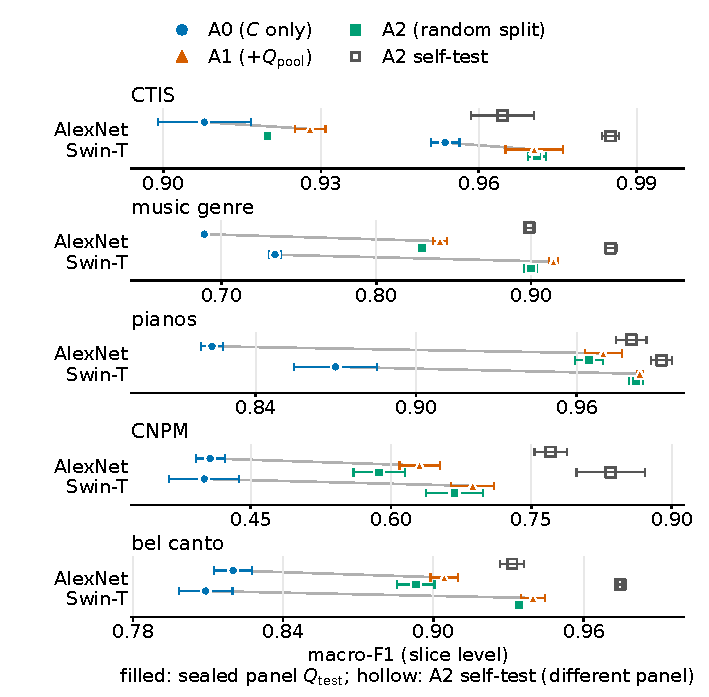
\includegraphics[width=\linewidth]{../figures/fig4_three_arms.pdf}
\caption{Sealed-panel macro-F1 at slice level for the three main arms; the five libraries form the
panels and the two backbones the rows. Circles: A0, which sees no test-adjacent content. Triangles: A1, into which the
held-out pool is injected by equal replacement. Filled squares: A2, our reconstruction of a
slice-level split.
Open squares: A2's own self-test score, drawn slightly above the row for legibility without
changing its horizontal value. It uses a different panel, not the sealed test panel.
Within each row the three arms are dodged vertically (A0 highest, A2 lowest) so that arms
whose scores coincide stay distinguishable; vertical position carries no quantitative meaning.
Horizontal whiskers are $\pm1$ sample standard deviation over three training seeds, not a
confidence interval and not the paired interval in Table~\ref{tab:main}. Horizontal segments span A0 to A1. Note that the horizontal axis is scaled per
library: the five baselines span 0.40 to 0.95, and a shared axis would compress the primary
library's two-point difference to invisibility.}
\label{fig:arms}
\end{figure}

\subsection{Near-single-slice controls as pipeline sanity checks}

Six A0 versus A2 contrasts on the three usable K$\approx$1 libraries, each with three seeds, give
five intervals that include zero, as Table~\ref{tab:neg} lists, and the intervals are narrow: apart from
one cell their outer bounds lie within about four points of zero. The remaining cell, chest\_falsetto
under Swin-T, is the only negative departure and the only interval that excludes zero
at $-2.53$ with CI $-5.00$ to $-0.21$; its per-seed deltas are $+5.57$, $-2.62$ and $-10.54$, so its 16.1-point
seed range is larger than the effect itself. The signs differ across the three trained seeds,
so this conditional interval does not establish a stable direction across training runs. The expansion from one
to three seeds was exploratory, not publicly preregistered. GZ\_IsoTech, the only control with multi-segment recordings, sits at $+0.26$ and $-0.22$,
consistent with its sub-one-percent exposure. Because A2 is not the main intervention, these cells
do not test A1$-$A0 directly and cannot bound uncertainty in the main experiment.
With six contrasts and no correction for multiplicity, the single nominal exclusion is itself weak
evidence, and five intervals that include zero do not show that the contrast is zero.
Recording- and slice-level partitions coincide only in the exactly single-slice collections,
so these are pipeline checks rather than evidence isolating a universal leakage mechanism.

\begin{table}[t]
\centering
\caption{Negative controls: A0 versus A2 on libraries with roughly one slice per recording, three
seeds. With one slice per recording there is no homologous content, so the exposure arm is not
identifiable and A2 is the only arm that can differ; the contrast column therefore measures protocol
noise rather than leakage. Five of the six intervals include zero. The remaining one is the only
negative departure, chest\_falsetto under Swin-T at $-2.53$, and its seed range of 16.1 points shows
substantial sensitivity to the three trained seeds. The six contrasts are reported without a
correction for multiplicity, and five intervals that include zero are not an equivalence test:
they do not establish that the protocol contrast is zero. This does not establish the cause of the
non-zero conditional interval. Intervals are 95\% recording-cluster bootstrap intervals
(2{,}000 resamples) conditional on the fixed seeds and split.}
\label{tab:neg}
\footnotesize
\setlength{\tabcolsep}{3.6pt}
\begin{tabular}{llrrrr}
\toprule
Library & Backbone & Rec.\, /\, slices & $\Delta$ [95\% CI] (pts) & Seed range (pts) & Tail prop. \\
\midrule
chest\_falsetto     & AlexNet & 1{,}280 / 1{,}280 & $-1.37\;[-3.31,+0.56]$ & 4.29  & 0.167 \\
chest\_falsetto     & Swin-T  & 1{,}280 / 1{,}280 & $-2.53\;[-5.00,-0.21]$ & 16.12 & 0.036 \\
erhu\_playing\_tech & AlexNet & 1{,}253 / 1{,}253 & $+0.03\;[-1.14,+1.24]$ & 2.54  & 0.928 \\
erhu\_playing\_tech & Swin-T  & 1{,}253 / 1{,}253 & $-0.49\;[-1.93,+0.40]$ & 1.93  & 0.382 \\
GZ\_IsoTech         & AlexNet & 2{,}824 / 2{,}899 & $+0.26\;[-0.23,+0.87]$ & 0.26  & 0.381 \\
GZ\_IsoTech         & Swin-T  & 2{,}824 / 2{,}899 & $-0.22\;[-0.56,+0.05]$ & 0.74  & 0.163 \\
\bottomrule
\end{tabular}
\end{table}

\subsection{Technique classification performance decreases on held-out instruments}

The cross-instrument experiment gives the largest contrast in the study and the one most
useful for interpreting published technique-classification numbers. With random slice-level
folds, pooled macro-F1 on CTIS techniques reaches 0.845 under AlexNet and 0.877 under Swin-T.
Grouping the folds by instrument --- same data, same budget, but every test recording's
instrument withheld from training --- brings the same pipeline to 0.448 and 0.530. The difference is $+39.6$ points
$[+36.8,+42.4]$ under AlexNet and $+34.8$ points $[+32.0,+38.1]$ under Swin-T, as
Table~\ref{tab:p3} reports.

Two things change between those two arms, so we added a third partition, R-rec, that
provides an operational intermediate comparison: folds are grouped by recording, with 110
instruments appearing on at least two folds. Thus most instrument overlap is retained while
recording overlap is removed, but not every instrument is present in every training/test pair.
Recording-grouped partitions are feasible on this corpus: no recording and no duplicate-audio group
crosses a fold, all 43 classes keep at least one test recording in the recording-grouped partition,
and fold sizes differ by less than 0.1\%. The instrument-withheld partition is tighter: its first
fold covers 42 of the 43 classes, because one technique class has no test recording there, and the
pooled metric averages only over classes present. The class universe itself comes from a
study-specific rule stated in Section~\ref{sec:protocol}: technique--instrument cells with at least
two recordings and instruments contributing at least three recordings, after excluding six
content-type labels. The R-rec partition reaches 0.816
and 0.843, so removing the recording-level leak lowers macro-F1 by $2.90$ points
(CI $0.32$ to $5.66$) under AlexNet and $3.41$ points (CI $0.68$ to $6.36$) under Swin-T.
Withholding the instruments then lowers it by a further $36.7$ points ($33.3$ to $39.9$) and
$31.4$ points ($28.3$ to $35.0$). The large number in
Table~\ref{tab:p3} is therefore two effects of very different size: within-instrument
the R-slice--R-rec contrast is 7--10\% of the total, with the larger remainder in the
R-rec--L-inst contrast. This separates protocol contrasts rather than decomposing
all sources of performance loss: neither the 36.7-point (AlexNet) or 31.4-point (Swin-T)
R-rec--L-inst gap nor the 39.6-point or 34.8-point R-slice--L-inst gap is a leakage estimate.
Figure~\ref{fig:p3} shows the
four partitions side by side with their intervals.

\begin{figure}[!tb]
\centering
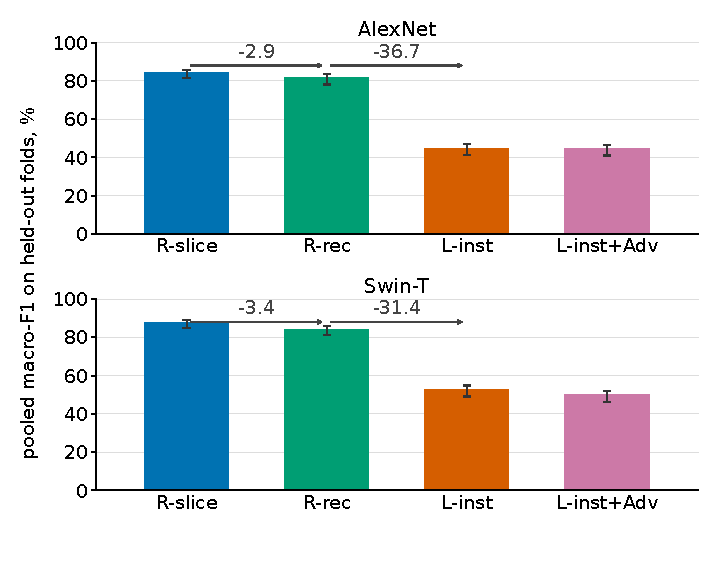
\includegraphics[width=\linewidth]{../figures/fig2_p3_decomposition.pdf}
\caption{Separating recording-disjoint and instrument-withheld protocol contrasts. Pooled macro-F1 on
held-out folds of the CTIS technique task for four partitions: random slice-level folds (R-slice),
recording-grouped folds with 110 instruments on at least two folds (R-rec),
instrument-withheld folds (L-inst), and the adversarial arm on the same folds (L-inst+Adv). Bars are means over
two seeds and the whiskers are 95\,\% recording-cluster bootstrap intervals. The two arrows
give the R-rec$--slice contrasts of $-2.9$ and $-3.4$ points and the
L-inst$--rec contrasts of $-36.7$ and $-31.4$ points, for AlexNet and Swin-T in that
order. They are differences between
protocols, not causal components of a single mechanism.}
\label{fig:p3}
\end{figure}

The adversarial instrument head does not recover the loss relative to L-inst. Under AlexNet it changes pooled
macro-F1 by $-0.36$ $[-1.75,+0.91]$; under Swin-T it changes it by $-2.83$ $[-4.81,-0.89]$.
The instrument-identity probe, fitted on a closed set of the instrument classes present in the
training recordings, shows that this information remains decodable: on frozen features
it reaches AUC 0.94 for R-slice and 0.96 for L-inst, and the adversarial head lowers it only
to 0.93 for L-inst+Adv while technique macro-F1 falls. Because the probe is fitted on an 80/20
split of the training recordings and its class set is closed, it measures how much instrument
identity remains recoverable for instruments the model has seen; it does not establish that an
unseen test instrument is identifiable from the representation. These rounded summaries are pooled across
folds, seeds and both backbones; Supplementary Material S1 gives the backbone-specific probe values.
The gradient-reversal weight was at most 0.02. The adversarial and L-inst arms use the same
instrument-grouped folds; they
differ in the objective, not the recordings seen.
This is a negative result for this intervention and weight schedule, not evidence that
instrument invariance is unattainable.

\begin{table}[t]
\centering
\caption{Cross-instrument transfer on CTIS techniques, over 43 classes, 1{,}388 recordings and
7{,}528 slices in three folds with two seeds, pooled over the held-out folds. R-slice uses random slice-level folds and
is the optimistic within-recording reference; R-rec groups folds by recording while retaining overlap for 110 instruments on at least two folds; L-inst withholds whole instruments; L-inst+Adv adds an adversarial instrument head on top of
L-inst. The recording-level column for R-slice aggregates slice predictions from more than one
fold model, so it is not directly comparable with the single-model recording-level column of the
other partitions. Intervals are 95\% recording-cluster bootstrap intervals. Contrasts on the pooled slice metric: R-slice$-$L-inst
$+39.63\,[+36.84,+42.39]$ for AlexNet and $+34.77\,[+32.00,+38.08]$ for Swin-T; R-slice$-$R-rec
$+2.90\,[+0.32,+5.66]$ and $+3.41\,[+0.68,+6.36]$; R-rec$-$L-inst
$+36.73\,[+33.31,+39.89]$ and $+31.37\,[+28.32,+34.97]$; L-inst+Adv$-$L-inst $-0.36\,[-1.75,+0.91]$ for AlexNet
and $-2.83\,[-4.81,-0.89]$ for Swin-T. Contrasts use unrounded scores and can
differ from the difference of the four-decimal columns by 0.01.}
\label{tab:p3}
\footnotesize
\setlength{\tabcolsep}{3.6pt}
\begin{tabular}{llrr}
\toprule
Arm & Backbone & Pooled macro-F1, slice & Pooled macro-F1, rec. \\
\midrule
R-slice         & AlexNet & 0.8446 & 0.8797 \\
R-slice         & Swin-T  & 0.8772 & 0.9041 \\
R-rec & AlexNet & 0.8157 & 0.8640 \\
R-rec & Swin-T  & 0.8431 & 0.8799 \\
L-inst & AlexNet & 0.4483 & 0.4917 \\
L-inst & Swin-T  & 0.5295 & 0.5676 \\
L-inst+Adv      & AlexNet & 0.4447 & 0.4714 \\
L-inst+Adv      & Swin-T  & 0.5012 & 0.5467 \\
\bottomrule
\end{tabular}
\end{table}

\subsection{Compute}

The final main comparison contains 60 A0/A1 training runs and 30 A2 runs. The expanded
negative controls contain 36 runs, the CTIS-only C1 control six runs, and the cross-instrument
experiment 48 fold-models including the recording-grouped intermediate arm. Driver timings
are rounded wall-clock batch durations on one 16 GB GPU, not independently metered GPU-hours.
Available logs indicate about 6.25 h for A0/A1, 4.15 h for A2, 2.99 h for the cross-instrument
fold-models and 1.17 h for C1; an additional recording-grouped/probe driver records about
0.55 h. Negative-control timing and abandoned exploratory runs are incompletely recoverable.
We therefore report the partial ledger in Supplementary Material S1, not an exact full-study
cost. Rebuilding recording identifiers and splits itself does not require a GPU.

\section{Discussion}\label{sec:discussion}

\subsection{What the size of the effect depends on}

The ten point estimates in Table~\ref{tab:main} differ across libraries and backbones. The
library medians of exposure are similar, but class-level exposures and other properties vary.
We did not fit an explanatory model or establish a variance decomposition, so we cannot determine
which factors explain the observed spread.

Headroom constrains the scale. A library whose control arm already reaches 0.95 cannot show a large
absolute gain, whatever the split does; CTIS loses at most 4.6 points to Swin-T and 9.2 to
AlexNet. In bel canto the recording-level control reaches the low 0.9s and the exposure arm
saturates at 1.00 for most seeds, so its recording-level contrast is limited by a ceiling and its
interval is wide for that reason as well as for the small panel of 40 test recordings.
Rescaling by headroom, as Table~\ref{tab:headroom} does, reduces but does not remove
the dispersion (0.219--0.873, still about four-fold): the normalised contrast is 22--37\% of the score headroom in CTIS, 38--48\% in
CNPM, 47--68\% in bel canto, 49--68\% in music genre, and 83--87\% in pianos. Absolute points
answer the question ``how much would the leaderboard move''; the rescaled number answers the
question ``how large is the contrast relative to the baseline's remaining score headroom''.
Because $1-\text{macro-F1}$ is not an error count, this is a descriptive normalised
effect size, not a division of predictions into memorisation and transfer.

The exposure ratio mainly reflects the chosen test share, half-pool allocation and training
budget, giving approximately 0.167. The five library medians range from 0.160 to 0.170, while
class-level values vary. These summaries alone cannot establish the role of exposure in the
between-library differences; task difficulty, class structure and recording similarity may also
matter, and our measurements do not isolate their contributions.

\subsection{Interpreting the primary result}

The internal plan identifies CTIS as the primary library because it is the largest and its class
structure supports the main design. There is no independent public timestamp establishing when
that choice was fixed. CTIS has the smallest observed absolute effects, with limited score
headroom for both backbones. Conditional intervals exclude zero, but only the Swin-T interval is
wholly below the study-specific three-point SESOI. These results distinguish statistical evidence
from practical importance; they do not establish the timing of the internal choice.

The four additional libraries show larger observed changes, from $+8.4$ to $+28.7$ points,
compared with $+2.02$ (AlexNet) and $+1.70$ (Swin-T) in CTIS. The tasks and class structures
differ, so these comparisons are descriptive.

The C1 control sharpens what the primary contrast can and cannot mean. It supplies the same volume
of training slices from non-test content, and the exposure arm still leads it by $+1.96$ points
under AlexNet ($+0.74$ to $+2.99$) and $+1.07$ under Swin-T ($+0.23$ to $+1.96$), so the
difference between the two arms is not explained by training volume. What survives is a contrast
that also changes the provenance of the injected content and the diversity of its recordings, which
the design does not separate: the A1--A0 difference is consistent with an advantage of
within-recording exposure, and it does not isolate one.

\subsection{What a reporting standard should require}

Four reporting practices would make evaluation protocols easier to interpret.

\emph{Name the split unit.} ``Randomly split 8:1:1'' is ambiguous only because the release format
makes slices look atomic. A statement of the form ``split by recording, 8:1:1 over recordings,
stratified by class'' identifies the intended unit; releasing the split assignments and grouping
rules allows the implementation to be checked.

\emph{Report the slice-per-recording distribution.} The distribution of $K$, not its mean alone,
determines the exposure probabilities under a specified slice-level split; the mean ranges from 8.7 to 48.9 across these
five libraries, so a single pooled statement about ``the dataset'' would be misleading even if
the split unit were named.

\emph{Report capacity when a stricter split is claimed.} If a paper says it splits by recording,
the reader needs to know whether that was feasible at the stated class counts: $q_c$,
$m_c$, and the resulting $\alpha_c$ document the constraints. CNPM and bel canto retain only
54 and 40 test recordings, respectively, so inference at recording level is especially uncertain. Our feasibility table is released with the splits precisely so that this
arithmetic can be checked rather than trusted.

\emph{Preserve the evaluation record.} Evaluating the held-out panel after training without
selecting on it limits selection bias, and stored predictions permit re-analysis. Our local
staging and sealing records do not independently establish when choices were made.

\subsection{Relation to prior audits}

Our result is consistent with Sturm~\cite{sturm2012gtzan} in kind and different in object: Sturm found
that a benchmark's content --- its labels and its duplicates --- did not support the conclusions drawn from it; we
show how one reconstruction of an ambiguously described evaluation recipe can affect scores.
The original realised split is unknown, so we cannot attribute the observed score change to that implementation.
The distinction matters for repair. Mislabelled audio has to be re-annotated; a
slice-level split can be rebuilt from recording identifiers if class capacity permits it, as
we demonstrate for the retained classes in these five libraries. Split construction itself is
CPU work; training costs are itemised separately in Section~\ref{sec:results}.

\subsection{Limitations and threats to validity}

\emph{One feature family.} We audited MEL only. The framework also releases chroma and CQT, and
the leakage mechanism is identical for them, but the magnitude need not be: chroma discards
timbre and may carry less recording identity.

\emph{What the contrast identifies.} A1 holds the training budget and the C-side recording
count fixed, but it does add pool recordings, so its training set contains more distinct
recordings than A0's. The contrast is therefore the effect of equal replacement under the
corpus's own composition --- the rule a reader applying this protocol would follow --- and not a
decomposition of memory into a content component and a diversity component. C1 addresses this
partly: equal-volume non-test injection changes macro-F1 by $+0.05$ and $+0.62$ points compared
with $+2.02$ and $+1.70$ for A1. C1 also changes recording diversity and uses R content; the
C1--A1 difference therefore cannot isolate a pure memorisation component.

\emph{Two backbones, three seeds.} The primary analysis uses AlexNet and Swin-T at seeds
0--2. The primary intervals condition on these runs; the supplementary joint bootstrap exposes
sensitivity to their dispersion, but three seeds cannot characterise the distribution of training
outcomes. We claim neither upper nor lower bounds for other architectures or training recipes.

\emph{One split realisation.} The recording-level split has a single seed. Capacity numbers are
computed for that realisation, and per-class exposure is reported rather than tested, because
the capacity table stores the mean of 400 random draws while a split realises one.

\emph{Reconstruction of the audited protocol.} We could not retrieve the framework's own split
files; the A2 arm reconstructs one slice-level interpretation of the stated 8:1:1 protocol and
may differ from the authors' actual choice of split unit, seed and stratification. The A1$-$A0
contrast does not depend on that reconstruction and is the primary contrast in the internal plan.

\emph{Version of record.} We checked the published split description in TISMIR 8(1),
pp. 22--38 (Section~\ref{sec:framework}). The original realised splits remain unavailable, so
our contrasts cannot be attributed numerically to the original authors' models.

\emph{External validity.} All five libraries are Chinese-music collections. Nothing in the
mechanism is language-specific. In the single-slice controls recording- and slice-level units
coincide by construction; the low-exposure control only approximates this condition. These
sanity checks are consistent with, but do not by themselves establish, slice multiplicity as the
operative explanation. The control libraries differ in task and classes, and one contrast excludes
zero. We do not claim that the magnitudes transfer to other benchmark suites without measurement.

\section{Conclusion}\label{sec:conclusion}

A benchmark that releases feature images rather than audio may make the split unit easy to lose. We
audited the unified evaluation framework of CCMusic, which states an 8:1:1 ratio for CTIS after
2-second segmentation without naming a unit, and rebuilt five MEL libraries --- 110{,}415 slices, 7{,}827
recordings, 252 source classes --- retaining 109{,}831 slices, 7{,}756 recordings and 234 classes
for recording-level analysis. Three main arms and the CTIS-only C1 control assess equal-volume
replacement rather than isolate a pure memory component: in the primary library, injecting the
held-out pool of test-adjacent slices by equal replacement raises macro-F1 by $+2.02$ points
with CI $+0.83$ to $+3.35$ under AlexNet and $+1.70$ with CI $+1.28$ to $+2.84$ under
Swin-T. The Swin-T interval lies below the internally specified three-point threshold;
AlexNet's upper limit of 3.35 does not exclude that magnitude. Against C1, which replaces the same
volume with non-test content, the exposure arm still leads by $+1.96$ and $+1.07$ points with
intervals that exclude zero. Four additional libraries show
$+8.4$ to $+28.7$ points. In near-single-slice controls five of six conditional intervals include
zero; the sixth excludes zero, but its three seed-specific effects differ in sign, and the six are
reported without a multiplicity correction. Dividing the A1$-$A0 contrasts by the baseline's score
headroom gives 22--87\%; this is a normalised effect size, not a decomposition into
memorisation and transfer, since $1-\text{macro-F1}$ is not an error count.
The division between memorisation and transfer is arguably not identifiable from these runs.

Two things follow for practice: report the split unit, the slice-per-recording distribution, and
the capacity arithmetic that makes a stricter split feasible; and seal the held-out panel so that
the resulting estimate can be re-derived from stored predictions.

The manifests, splits, sealed predictions and analysis code supporting the reported results are
openly available at \url{https://github.com/ristar2018/ccmusic-split-audit}. Supplementary
Material S1 documents the reconstruction and execution history. The verification script checks
the reported tables against stored artifacts; recomputation of bootstrap summaries uses the
separate analysis scripts and needs no new training.

\section*{Statements and Declarations}

\subsection*{Funding}

This research was supported by the Xinxiang Social Science Federation Research Project (2026,
Grant No.\ SKL-2026-0504).

\subsection*{Competing interests}

The authors have no relevant financial or non-financial interests to disclose.

\subsection*{Data availability}

The underlying libraries are publicly released by the CCMusic project; we do not redistribute
them, and they remain under the terms of their original release. The recording manifests, the
recording-level splits, the sealed predictions, the analysis
code and the verification script required to reproduce every table and figure are openly
available at \url{https://github.com/ristar2018/ccmusic-split-audit}. The repository also carries
the design plan, the execution-change list and the expected verification output. The feature cache is a derived artifact --- 224$\times$224 resized copies of the released MEL
images --- and is not redistributed: at 16.24 GiB it does not belong in a code repository, and
it can be rebuilt from the released images with the script provided. The
released derived material therefore consists of manifests, split definitions, predictions and
the index files that record the cache contents; it contains no audio, no source images and
nothing else that could substitute for the original libraries. The manuscript describes the state of that repository at
the commit recorded in \texttt{docs/execution-changes.md}, and the accompanying release package
pins the same files by checksum.

\subsection*{Author contributions}

\textbf{Yuan Zhao:} Conceptualization, Methodology, Formal analysis, Writing -- review \& editing,
Project administration. \textbf{Yingtao Ji:} Data curation, Formal analysis, Investigation,
Methodology, Writing -- original draft, Writing -- review \& editing, Funding acquisition.
\textbf{Mengjie Hu:} Software, Methodology, Formal analysis, Investigation.
\textbf{Songmei Liu:} Validation, Writing -- review \& editing, Supervision.
\textbf{Chenyu Yang:} Data curation, Investigation, Validation.
All authors have read and approved the final manuscript.

\subsection*{Ethics approval}

Not applicable. The study analyses publicly released datasets; it involves no human participants,
no animals, and no personally identifiable information.

\subsection*{Reproducibility and verification}

The numerical verifier checks artifact identities, recalculates seed means and differences,
and compares generated table rows with the manuscript. Bootstrap intervals are produced by
separate scripts from sealed predictions; the verifier does not independently rerun every
bootstrap or validate every prose claim. Supplementary Material S1 records the environment,
commands, execution changes, supplementary analyses and known gaps. The design was documented
internally and was not publicly preregistered. Each training run writes its own log and its own validation curve, and every driver script
skips completed runs, so an interrupted batch resumes by re-issuing the same command.

\begin{sloppypar}
\noindent\textbf{Artifacts.}
Splits: \texttt{data/splits/v2/} covering eight libraries, with \texttt{assertions.json},
\texttt{feasibility.csv} and \texttt{splits\_hash.json}.
Feature cache: \texttt{data/cache/mel224/} with 115{,}847 images, 16.24 GiB, and
\texttt{CACHE.json}; the cache covers the released images of all audited libraries, including the
images of classes excluded by the minimum-recording rule, plus the 5{,}432 control images.
Sealed predictions: \texttt{runs/sealed\_eval/}, holding \texttt{.npz} archives with per-slice
probabilities, labels and recording indices.
Cross-instrument archive: \texttt{runs\_p3/}.
Result tables: \texttt{data/results/}.
\end{sloppypar}


\bibliography{refs}

\end{document}
